% Copyright (C) 2017 - Michael Baudin

  \documentclass{beamer}

%\setbeameroption{hide notes}
%\setbeameroption{show notes}
%\setbeameroption{show only notes}

  % Copyright (C) 2012 - EDF R&D - Michael Baudin

% To highlight source code
\usepackage{listings}
\definecolor{darkgreen}{rgb}{0,0.5,0}
\definecolor{violet}{rgb}{0.5,0,1}

\usepackage{lmodern}% http://ctan.org/pkg/lm

\usetheme{Montpellier}
\setbeamertemplate{navigation symbols}{} % Remove navigation
\useoutertheme{infolines}

\usepackage[utf8]{inputenc}
\usepackage[T1]{fontenc}

%\usepackage[french]{babel}
%\uselanguage{French}
%\languagepath{French}

\def\bx{{\bf x}}
\def\RR{\mathbb{R}}

\newcommand{\pyvar}[1]{\texttt{#1}}

\def \ot {OpenTURNS}

\hypersetup{colorlinks=true}


\title[OpenTURNS's GUI]{The graphical user interface of OpenTURNS, a UQ software in simulation}

\author[Baudin et al.]{
Micha�l Baudin \inst{1} \and
Anne Dutfoy \inst{1} \and
Anthony Geay \inst{1} \and
Anne-Laure Popelin \inst{1} \and
Aur�lie Ladier \inst{2} \and
Julien Schueller \inst{2} \and
Thierry Yalamas \inst{2}
}

\institute[EDF-Phim�ca]{
\inst{1} EDF R\&D. 6, quai Watier, 78401, Chatou Cedex - France, michael.baudin@edf.fr \and %
\inst{2} Phimeca Engineering. 18/20 boulevard de Reuilly, 75012 Paris - France, yalamas@phimeca.com
}

\date[]{15 June 2017, UNCECOMP 2017, Rhodes, Greece}

%%%%%%%%%%%%%%%%%%%%%%%%%%%%%%%%%%%%%%%%%%%%%%%%%%%%%%%%%%%%%%%%%%%%%%%%%%%%%

  \begin{document}

%%%%%%%%%%%%%%%%%%%%%%%%%%%%%%%%%%%%%%%%%%%%%%%%%%%%%%%%%%%%%%%%%%%%%%%%%%%%%

  \begin{frame}
  \titlepage
  
  \begin{columns}
    \column{0.45\textwidth}
  \begin{center}

\includegraphics[height=0.15\textheight]{figures/edf.jpg}
\end{center}
    \column{0.1\textwidth}
	
    \column{0.45\textwidth}
  \begin{center}

\includegraphics[height=0.15\textheight]{figures/logo_phimeca.png}
\end{center}
  \end{columns}

  \end{frame}

%%%%%%%%%%%%%%%%%%%%%%%%%%%%%%%%%%%%%%%%%%%%%%%%%%%%%%%%%%%%%%%%%%%%%%%%%%%%%

\begin{frame}
\frametitle{Contents}
\tableofcontents
\end{frame}

%%%%%%%%%%%%%%%%%%%%%%%%%%%%%%%%%%%%%%%%%%%%%%%%%%%%%%%%%%%%%%%%%%%%%%%%%%%%%
\section{Introduction}

%%%%%%%%%%%%%%%%%%%%%%%%%%%%%%%%%%%%%%%%%%%%%%%%%%%%%%%%%%%%%%%%%%%%%%%%%%%%%

\begin{frame}
\frametitle{\ot{}}

  \begin{columns}
    \column{0.6\textwidth}
	
\begin{itemize}
\item Uncertainty quantification, uncertainty propagation, sensitivity analysis and metamodeling
\item Partners : EDF, Phim�ca, Airbus, IMACS
\item \url{www.openturns.org}
\item Licence LGPL 
\item Linux, Windows
\end{itemize}

Programming:
\begin{itemize}
\item Python module
\item C++ Library
\end{itemize}

    \column{0.4\textwidth}

	\begin{center}
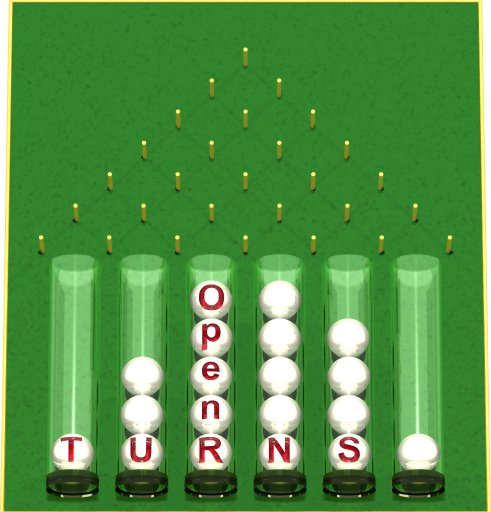
\includegraphics[width=0.9\textwidth]{figures/logo-ot}
\end{center}

	\end{columns}
\end{frame}

%%%%%%%%%%%%%%%%%%%%%%%%%%%%%%%%%%%%%%%%%%%%%%%%%%%%%%%%%%%%%%%%%%%%%%%%%%%%%

\begin{frame}
\frametitle{SALOME}

  \begin{columns}
    \column{0.5\textwidth}
	
\begin{itemize}
\item Integration platform for pre and post processing, and 2D/3D numerical simulation 
\item Features : geometry, mesh, distributed computing
\item Visualization, data assimilation, uncertainty treatment
\item Partners : EDF, CEA, Open Cascade
\item Licence : LGPL
\item Linux, Windows
\item \url{www.salome-platform.org}
\end{itemize}

    \column{0.5\textwidth}

	\begin{center}
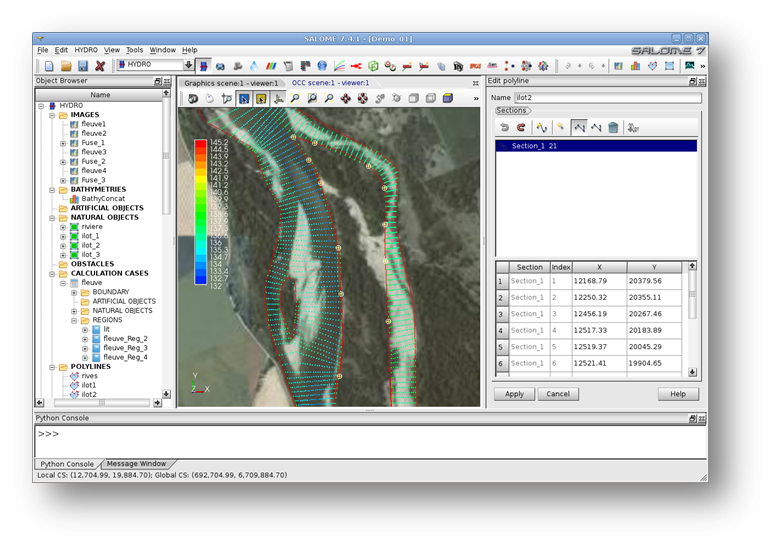
\includegraphics[width=0.95\textwidth]{figures/Salome-hydro-platform}
\end{center}

	\end{columns}
\end{frame}

%%%%%%%%%%%%%%%%%%%%%%%%%%%%%%%%%%%%%%%%%%%%%%%%%%%%%%%%%%%%%%%%%%%%%%%%%%%%%

\begin{frame}
\frametitle{The graphical user interface of \ot{}}
	
\begin{itemize}
\item Main goal : provide a graphical interface of 
\ot{} in SALOME
\item Features
	\begin{itemize}
	\item Uncertainty quantification (distribution fitting), 
	central tendency, sensitivity analysis, probability estimate, 
	meta-modeling
	\item Generic (not dedicated to a specific application)
	\item GUI language : English, French
	\end{itemize}

\item Partners : EDF, Phim�ca
\item Licence : LGPL

\item Schedule : 
	\begin{itemize}
	\item Since summer 2016, one EDF release per year
	\item On the internet : 2018
	\end{itemize}

\end{itemize}

\end{frame}

%%%%%%%%%%%%%%%%%%%%%%%%%%%%%%%%%%%%%%%%%%%%%%%%%%%%%%%%%%%%%%%%%%%%%%%%%%%%%

\section{Demo}

\begin{frame}
\frametitle{GUI : the demo}

\begin{center}
Demo time.
\end{center}

\end{frame}

%%%%%%%%%%%%%%%%%%%%%%%%%%%%%%%%%%%%%%%%%%%%%%%%%%%%%%%%%%%%%%%%%%%%%%%%%%%%%


\begin{frame}
\frametitle{GUI : outline}

\begin{itemize}
\item From scratch : 3 inputs, 2 outputs, sum, central dispersion study with default parameters
\item Open axialStressedBeam-python.xml : central dispersion with sample size 1000, Threshold P(G<0) with CV=0.05
\item Import crue-4vars-analytique.py : S.A. with sample size 1000, sort by size
\end{itemize}

\end{frame}


%%%%%%%%%%%%%%%%%%%%%%%%%%%%%%%%%%%%%%%%%%%%%%%%%%%%%%%%%%%%%%%%%%%%%%%%%%%%%
\section{Background}

\begin{frame}
\frametitle{UQ, the easy way}

Main goal : make UQ easy to use
\begin{itemize}
\item classical user-friendly algorithms with a 
state-of-the-art implementation,
\item default parameters of the algorithms whenever possible,
\item an easy access to the HPC resources,
\item an automated connection to the computer code.
\end{itemize}

Produce standard results :
\begin{itemize}
\item numerical results e.g. tables,
\item classical graphics.
\end{itemize}

\end{frame}

%%%%%%%%%%%%%%%%%%%%%%%%%%%%%%%%%%%%%%%%%%%%%%%%%%%%%%%%%%%%%%%%%%%%%%%%%%%%%

\begin{frame}
\frametitle{Overview (1/2)}

Inputs from the user :
\begin{itemize}
\item Physical model : symbolic, Python code or SALOME component
\item Probabilistic model : joint probability distribution function of the input.
\end{itemize}

Then :
\begin{itemize}
\item Central dispersion: estimates the central dispersion of the output Y (e.g. mean).
\item Threshold probability: estimates the probability that the output exceeds a given
threshold S.
\item Sensitivity analysis: estimates the importance of the inputs to the variability of the output.
\end{itemize}

\end{frame}

%%%%%%%%%%%%%%%%%%%%%%%%%%%%%%%%%%%%%%%%%%%%%%%%%%%%%%%%%%%%%%%%%%%%%%%%%%%%%

\begin{frame}
\frametitle{Overview (2/2)}

Probabilistic modeling :
\begin{itemize}
\item Distribution fitting from a sample
\item Dependence modeling (Gaussian copula)
\end{itemize}

Meta-modeling :
\begin{itemize}
\item Polynomial chaos (full or sparse)
\item Kriging
\end{itemize}

\end{frame}


%%%%%%%%%%%%%%%%%%%%%%%%%%%%%%%%%%%%%%%%%%%%%%%%%%%%%%%%%%%%%%%%%%%%%%%%%%%%%
\section{What's next ?}


\begin{frame}
\frametitle{Fields}
  \begin{columns}
    \column{0.5\textwidth}

Field example : 
\begin{itemize}
\item Input : 4 independent random variables
\item Output : height of the river Garonne on a 100 km segment
\item Computer code : TELEMAC2D
\item Quantity of interest : pointwise average over 70 000 random simulations
\end{itemize}

Roadmap : 
\begin{itemize}
\item Now : massive Python/\ot{} scripting
\item 2017-2018 : in the gui
\end{itemize}

    \column{0.5\textwidth}

\begin{center}
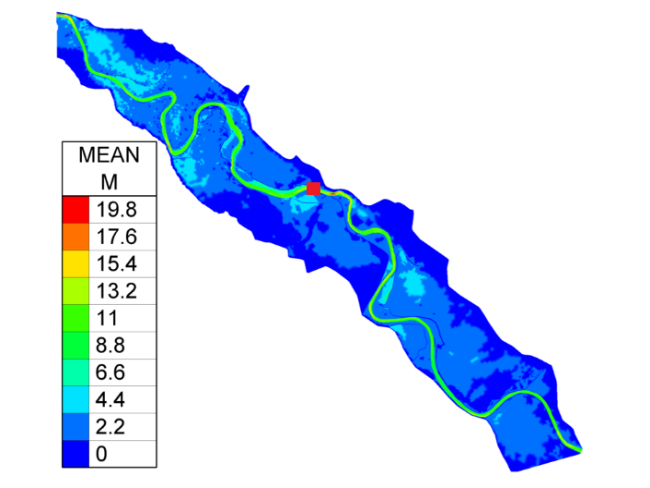
\includegraphics[height=0.5\textheight]{figures/image034.png}
\end{center}


	\end{columns}

\end{frame}

%%%%%%%%%%%%%%%%%%%%%%%%%%%%%%%%%%%%%%%%%%%%%%%%%%%%%%%%%%%%%%%%%%%%%%%%%%%%%

\begin{frame}
\frametitle{The end}

\begin{center}
Thanks !
\end{center}

\begin{center}
Questions ?
\end{center}

\end{frame}

%%%%%%%%%%%%%%%%%%%%%%%%%%%%%%%%%%%%%%%%%%%%%%%%%%%%%%%%%%%%%%%%%%%%%%%%%%%%%
\section{Extra slides}

\begin{frame}
\frametitle{Interactive uncertainty visualization with Paraview}

\begin{center}
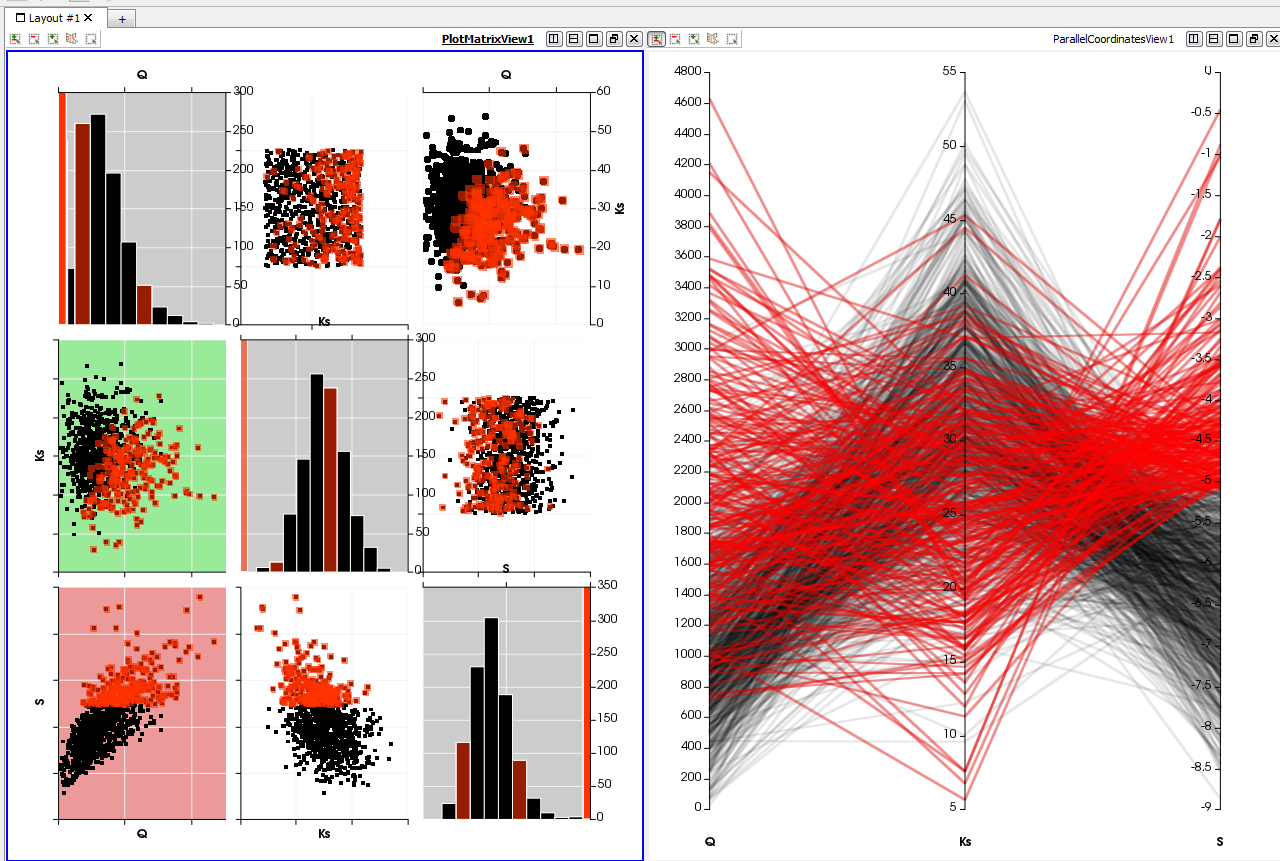
\includegraphics[width=0.9\textwidth]{figures/image032.png}
\end{center}

\end{frame}

%%%%%%%%%%%%%%%%%%%%%%%%%%%%%%%%%%%%%%%%%%%%%%%%%%%%%%%%%%%%%%%%%%%%%%%%%%%%%

\begin{frame}
\frametitle{Methodology}

\begin{center}
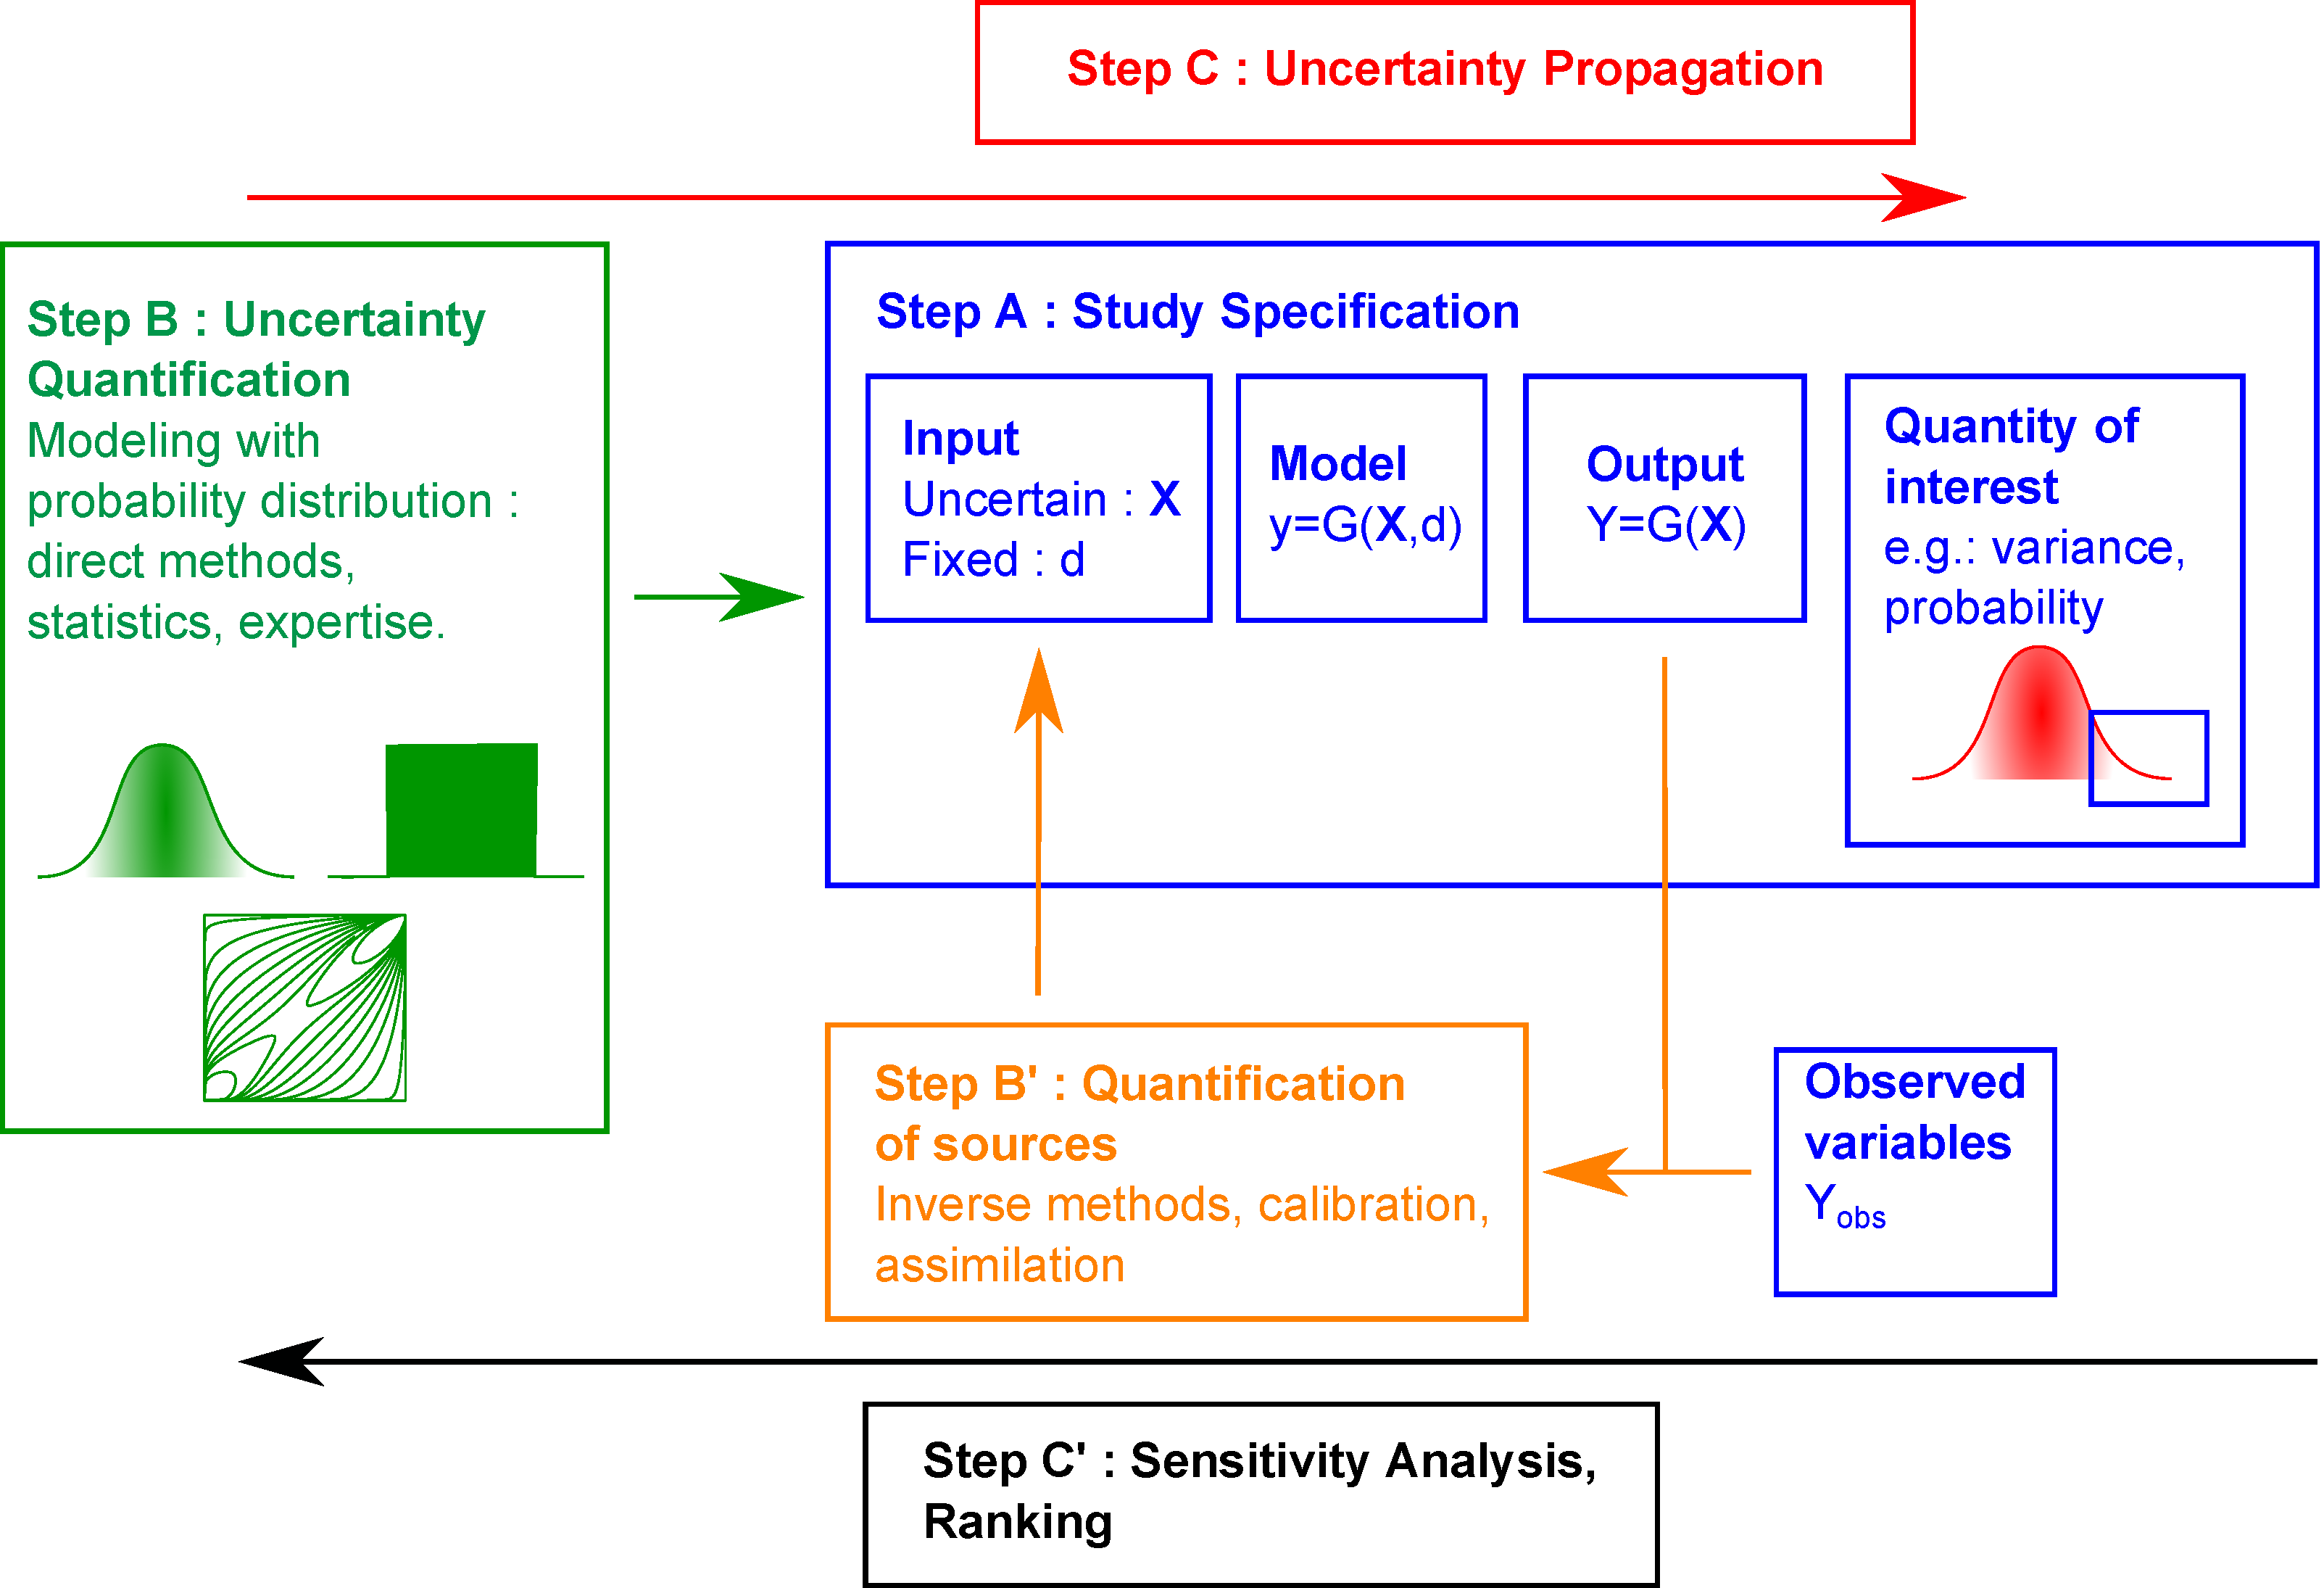
\includegraphics[width=0.9\textwidth]{figures/MethodologieIncertitude-EN.pdf}
\end{center}

\end{frame}

%%%%%%%%%%%%%%%%%%%%%%%%%%%%%%%%%%%%%%%%%%%%%%%%%%%%%%%%%%%%%%%%%%%%%%%%%%%%%

\begin{frame}
\frametitle{Software architecture}

  \begin{columns}
    \column{0.4\textwidth}
	
Two entry points:
\begin{itemize}
\item interactive,
\item Python.
\end{itemize}

Advantages of the Python programming of the GUI:
\begin{itemize}
\item unit tests,
\item going beyond the GUI
\end{itemize}

    \column{0.6\textwidth}

\begin{center}
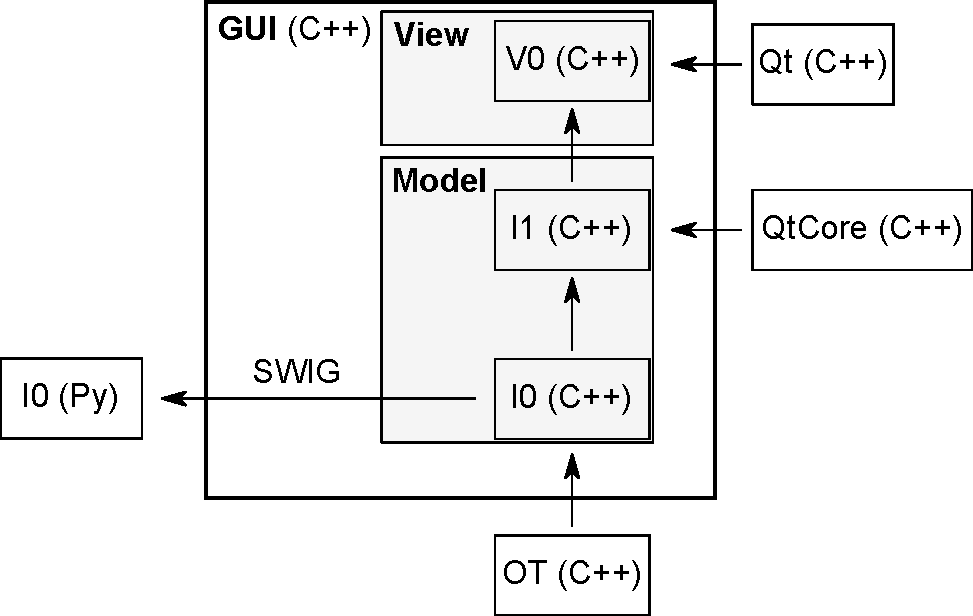
\includegraphics[width=0.95\textwidth]{figures/ArchiGUI-Internal.pdf}
\end{center}

	\end{columns}

\begin{center}
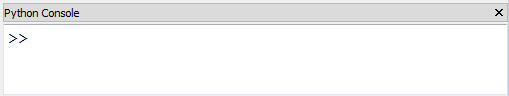
\includegraphics[width=0.9\textwidth]{figures/image007.png}
\end{center}

\end{frame}

%%%%%%%%%%%%%%%%%%%%%%%%%%%%%%%%%%%%%%%%%%%%%%%%%%%%%%%%%%%%%%%%%%%%%%%%%%%%%
\section{Demo backup}

%%%%%%%%%%%%%%%%%%%%%%%%%%%%%%%%%%%%%%%%%%%%%%%%%%%%%%%%%%%%%%%%%%%%%%%%%%%%%

\begin{frame}
\frametitle{Symbolic physical model}

\begin{center}
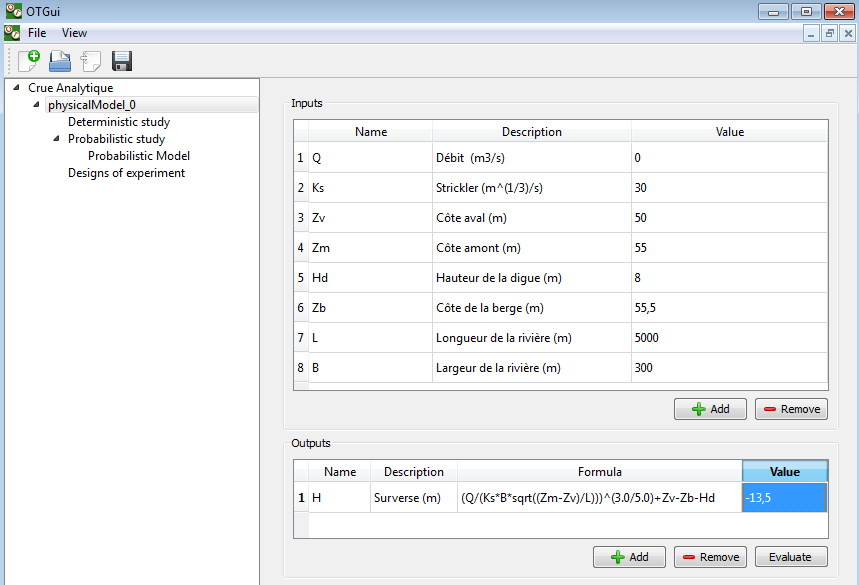
\includegraphics[width=0.9\textwidth]{figures/image009.png}
\end{center}

\end{frame}

%%%%%%%%%%%%%%%%%%%%%%%%%%%%%%%%%%%%%%%%%%%%%%%%%%%%%%%%%%%%%%%%%%%%%%%%%%%%%

\begin{frame}
\frametitle{Probabilistic model}

\begin{center}
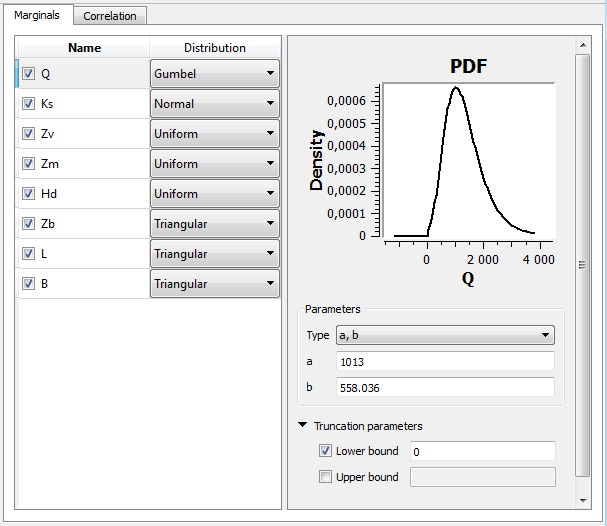
\includegraphics[height=0.8\textheight]{figures/image013.png}
\end{center}

\end{frame}

%%%%%%%%%%%%%%%%%%%%%%%%%%%%%%%%%%%%%%%%%%%%%%%%%%%%%%%%%%%%%%%%%%%%%%%%%%%%%

\begin{frame}
\frametitle{Limit state study : definition of the threshold}

\begin{center}
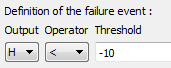
\includegraphics[width=0.4\textwidth]{figures/image015.png}
\end{center}

\end{frame}

%%%%%%%%%%%%%%%%%%%%%%%%%%%%%%%%%%%%%%%%%%%%%%%%%%%%%%%%%%%%%%%%%%%%%%%%%%%%%

\begin{frame}
\frametitle{Limit state study : algorithm parameters}

\begin{center}
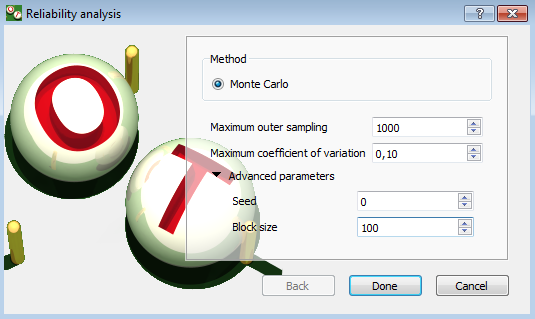
\includegraphics[width=0.95\textwidth]{figures/image017.png}
\end{center}

\end{frame}

%%%%%%%%%%%%%%%%%%%%%%%%%%%%%%%%%%%%%%%%%%%%%%%%%%%%%%%%%%%%%%%%%%%%%%%%%%%%%

\begin{frame}
\frametitle{Limit state study : summary}

\begin{center}
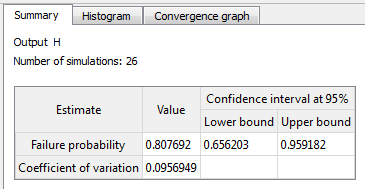
\includegraphics[width=0.7\textwidth]{figures/image019.png}
\end{center}

\end{frame}

%%%%%%%%%%%%%%%%%%%%%%%%%%%%%%%%%%%%%%%%%%%%%%%%%%%%%%%%%%%%%%%%%%%%%%%%%%%%%

\begin{frame}
\frametitle{Limit state study : histogram}

\begin{center}
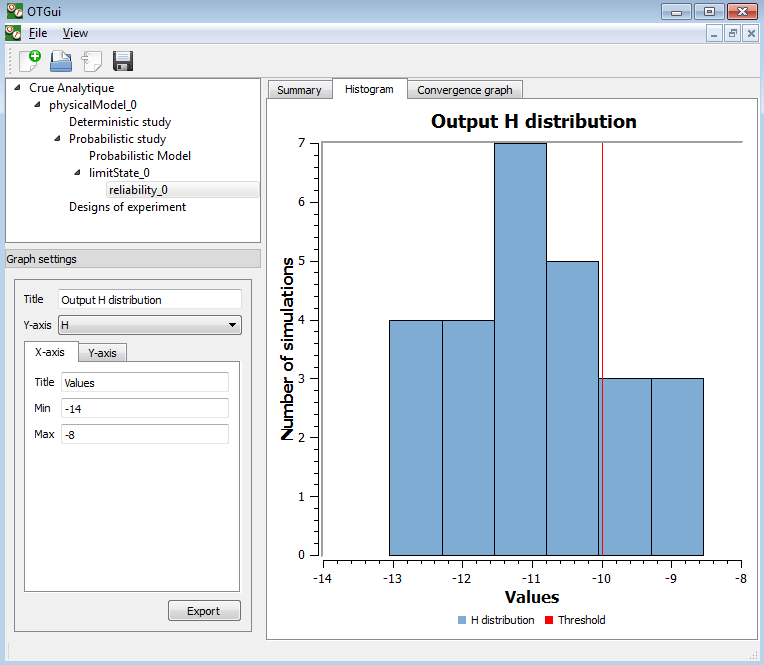
\includegraphics[width=0.7\textwidth]{figures/image021.png}
\end{center}

\end{frame}

%%%%%%%%%%%%%%%%%%%%%%%%%%%%%%%%%%%%%%%%%%%%%%%%%%%%%%%%%%%%%%%%%%%%%%%%%%%%%

\begin{frame}
\frametitle{Central tendency : algorithm parameters}

\begin{center}
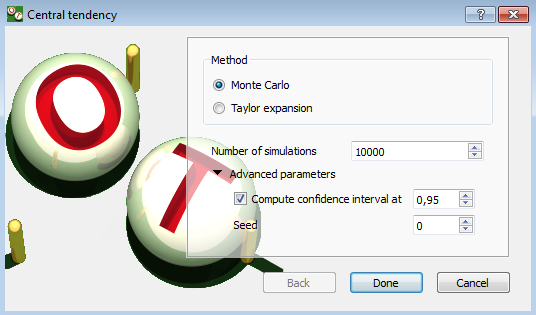
\includegraphics[width=0.8\textwidth]{figures/image023.png}
\end{center}

\end{frame}

%%%%%%%%%%%%%%%%%%%%%%%%%%%%%%%%%%%%%%%%%%%%%%%%%%%%%%%%%%%%%%%%%%%%%%%%%%%%%

\begin{frame}
\frametitle{Central tendency : summary results}

\begin{center}
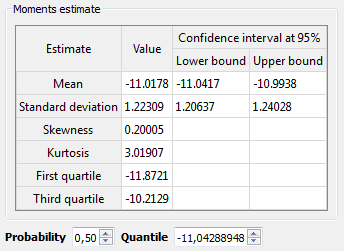
\includegraphics[width=0.8\textwidth]{figures/image025-bottom.png}
\end{center}

\end{frame}

%%%%%%%%%%%%%%%%%%%%%%%%%%%%%%%%%%%%%%%%%%%%%%%%%%%%%%%%%%%%%%%%%%%%%%%%%%%%%

\begin{frame}
\frametitle{Central tendency : summary results}

\begin{center}
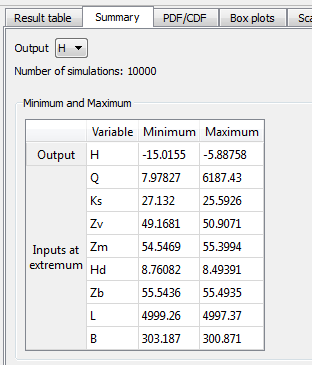
\includegraphics[height=0.8\textheight]{figures/image025-top.png}
\end{center}

\end{frame}

%%%%%%%%%%%%%%%%%%%%%%%%%%%%%%%%%%%%%%%%%%%%%%%%%%%%%%%%%%%%%%%%%%%%%%%%%%%%%

\begin{frame}
\frametitle{Central tendency : scatter plots}

\begin{center}
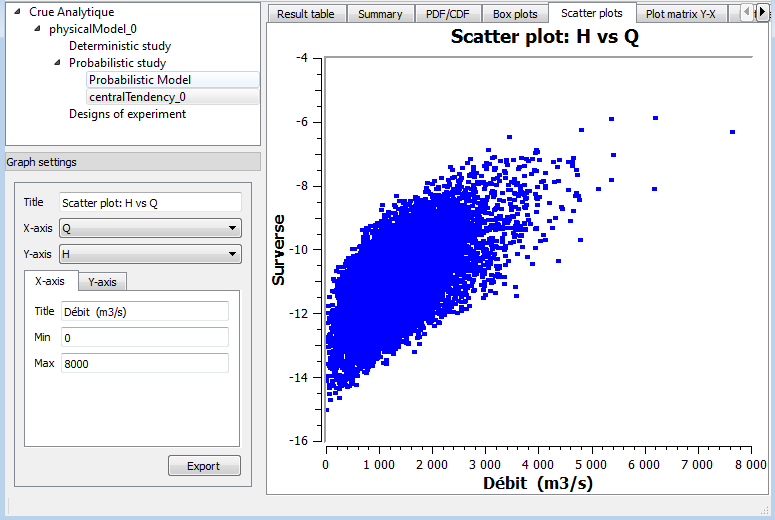
\includegraphics[width=0.8\textwidth]{figures/image028.png}
\end{center}

\end{frame}


%%%%%%%%%%%%%%%%%%%%%%%%%%%%%%%%%%%%%%%%%%%%%%%%%%%%%%%%%%%%%%%%%%%%%%%%%%%%%

\begin{frame}
\frametitle{Sensitivity analysis : Sobol' indices}

\begin{center}
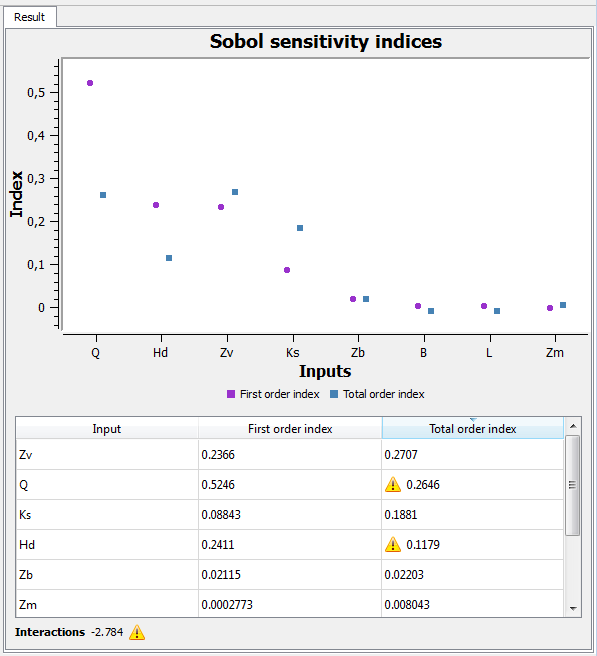
\includegraphics[height=0.8\textheight]{figures/image030.png}
\end{center}

\end{frame}

\end{document}
